\documentclass[sigconf,nonacm]{acmart}
\settopmatter{printacmref=false}
\setcopyright{none}
\renewcommand\footnotetextcopyrightpermission[1]{}
\acmConference[Course Project]{Analysis of Algorithms: Project 2}{November 2026}{}
\acmDOI{}
\acmISBN{}
\usepackage{amsmath}
\usepackage{amsthm}
\usepackage{algorithm}
\usepackage{algpseudocode}
\usepackage{tikz}
\usetikzlibrary{arrows.meta,positioning}
\usepackage{pgfplots}
\pgfplotsset{compat=1.18}
\usepackage{listings}
\usepackage{fvextra}
\newtheorem{theorem}{Theorem}
\newtheorem{lemma}{Lemma}
\lstset{language=Python,basicstyle=\ttfamily\scriptsize,
  breaklines=true,columns=fullflexible,keepspaces=true,
  numbers=left,numberstyle=\tiny,numbersep=5pt,showstringspaces=false}
\input{../results/summary.tex}
\title{Staffing Volunteers and Locating Emergency Supply Depots:\\
Exact Network Flow and Greedy Set Cover}
\author{Student One --- replace before submission}
\affiliation{\institution{Course institution --- replace before submission}\country{}}
\author{Student Two --- replace or remove for an individual submission}
\affiliation{\institution{Course institution --- replace before submission}\country{}}
\begin{document}
\begin{abstract}
Two public-service planning tasks illustrate different algorithmic approaches.
Volunteer staffing is modeled as a bipartite eligibility graph with workload
limits and shift demands. We construct a capacitated network and prove that
an integral flow saturating the demand arcs exists exactly when a complete
assignment exists. A full Edmonds--Karp implementation returns an assignment
or certifies that full staffing is impossible. Emergency supply depot selection
is modeled by an explicit site--community coverage relation. Its decision
version is NP-complete by a reduction from Set Cover; its optimization version
is NP-hard. A greedy coverage algorithm has a harmonic approximation guarantee.
Seeded synthetic experiments measure runtime and operation counts, and small
instances are checked against exhaustive solutions. All numerical results
come from the supplied executable experiment, with source code and an LLM-use
record provided in the appendices.
\end{abstract}
\keywords{network flow, volunteer assignment, NP-completeness, set cover, greedy algorithms}
\maketitle

\section{Introduction}
Public-service planners must allocate limited resources while meeting service
requirements. Two concrete examples are filling volunteer shifts and choosing
where to open emergency supply depots. The American Red Cross provides shift
sign-ups through Volunteer Connection~\cite{redcross}. FEMA's distribution
planning material describes commodity points of distribution as locations
through which survivors obtain supplies~\cite{fema}. These operational settings,
rather than an algorithms textbook, motivate our problem choices. We introduce
the following mathematical models as simplified planning models; the cited
organizations did not supply the instances or endorse the assumptions.

The first task assigns available, eligible volunteers to a fixed set of
nonoverlapping shifts. Volunteers have upper workload limits, and shifts have
fixed staffing requirements. The second task chooses a minimum-size collection
of candidate depots covering every community in a supplied coverage table.
The first admits an exact polynomial algorithm; the second contains Set Cover.
This difference persists even though both tasks can be represented as
bipartite graphs.

Our contributions are two explicit abstractions, polynomial constructions with
both directions of their correctness proofs, complete pseudocode, and tested
Python implementations. For the depot problem, we distinguish proving
NP-hardness from showing membership in NP. We also report controlled runtime
experiments and a small-instance assessment of greedy solution quality.

\section{Volunteer Staffing by Network Flow}
\subsection{Real task and abstraction}
Suppose an event coordinator must fill distinct time slots. Each shift has one
interchangeable role, every volunteer assigned to that shift can perform it,
and a volunteer may work on several shifts. Shifts do not overlap, so temporal
conflicts are already excluded. Any required training and availability are
encoded in eligibility. We omit preferences, travel between shifts, minimum
volunteer workloads, and consecutive-work constraints.

Let $W=\{w_1,\ldots,w_a\}$ be volunteers and
$J=\{j_1,\ldots,j_b\}$ be shifts. Let $R\subseteq W\times J$ be the
eligibility relation, $q=|R|$, $\ell_i\in\mathbb Z_{\ge0}$ a volunteer's
maximum number of shifts, and $d_j\in\mathbb Z_{\ge0}$ the required staffing
of a shift. Define total demand $D=\sum_j d_j$. A valid complete assignment is
a subset $A\subseteq R$ satisfying
\begin{align}
 |\{j:(w_i,j)\in A\}|&\le\ell_i &&\text{for every }i,\\
 |\{i:(w_i,j)\in A\}|&=d_j &&\text{for every }j.
\end{align}
Because $A$ is a set, the same volunteer cannot fill two positions on the same
shift. The output is such an assignment, or an infeasibility declaration.

\subsection{Polynomial construction}
Create vertices $\{s,t\}\cup W\cup J$ with the following directed arcs:
\begin{enumerate}
\item $s\to w_i$ with capacity $\ell_i$ for each volunteer;
\item $w_i\to j$ with capacity $1$ for each $(w_i,j)\in R$;
\item $j\to t$ with capacity $d_j$ for each shift.
\end{enumerate}
Thus $N=a+b+2$ and $M=a+b+q$. The mathematical construction takes
$O(N+M)$ time from adjacency lists and copies binary capacities without
expanding them into individual units. Its encoding length is polynomial in
the original input length, including capacity bit lengths. Decide feasibility
by testing whether the maximum flow value equals $D$.

\begin{figure}[t]
\centering
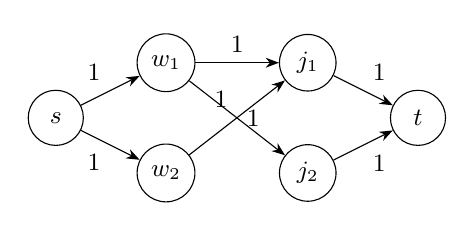
\begin{tikzpicture}[>=Stealth, every node/.style={font=\small},
  vertex/.style={draw,circle,minimum size=7mm}]
\node[vertex] (s) at (0,0) {$s$};
\node[vertex] (a) at (1.4,.7) {$w_1$};
\node[vertex] (b) at (1.4,-.7) {$w_2$};
\node[vertex] (x) at (3.2,.7) {$j_1$};
\node[vertex] (y) at (3.2,-.7) {$j_2$};
\node[vertex] (t) at (4.6,0) {$t$};
\draw[->] (s)--node[above left] {1}(a);
\draw[->] (s)--node[below left] {1}(b);
\draw[->] (a)--node[above] {1}(x);
\draw[->] (a)--node[right] {1}(y);
\draw[->] (b)--node[above left] {1}(x);
\draw[->] (x)--node[above right] {1}(t);
\draw[->] (y)--node[below right] {1}(t);
\end{tikzpicture}
\caption{A two-volunteer instance. A complete assignment is
$\{(w_1,j_2),(w_2,j_1)\}$. Labels are capacities.}
\label{fig:network}
\end{figure}

\subsection{Correctness of the reduction}
\begin{theorem}
A complete volunteer assignment exists if and only if the constructed network
has a flow of value $D$.
\end{theorem}
\begin{proof}
Suppose $A$ is a complete assignment. Put one unit on $w_i\to j$ for each
pair in $A$ and zero on the other eligibility arcs. Put the number of assigned
shifts of $w_i$ on $s\to w_i$, and put $d_j$ on $j\to t$.
The workload limits bound the first arcs, the fact that $A$ is a set bounds
the middle arcs, and the staffing equalities bound the last arcs. Flow is
conserved at every volunteer and shift. Its value is $D$.

Conversely, suppose a flow of value $D$ exists. Since capacities are integers,
an integral maximum flow exists; Edmonds--Karp, starting from zero, produces
one by integral augmentations. No flow exceeds $D$ because the total capacity
entering $t$ is $D$. Therefore an integral maximum flow has value $D$ and
saturates every arc $j\to t$. Select exactly the eligibility arcs carrying
one unit. Unit capacities make each selected pair unique. Conservation at a
volunteer and capacity $\ell_i$ give its workload bound. Conservation at a
shift and saturation of its sink arc give exactly $d_j$ volunteers. The
selected pairs form a complete assignment.
\end{proof}

\subsection{Complete algorithm}
Algorithm~\ref{alg:flow} includes the reduction and the maximum-flow procedure.
Each original arc has a reverse residual arc of initial capacity zero.
Updating reverse arcs allows earlier assignments to be revised. In
Figure~\ref{fig:network}, choosing $w_1\to j_1$ first is repaired by the
residual path $s,w_2,j_1,w_1,j_2,t$. Omitting reverse arcs would incorrectly
reject this feasible instance.

\begin{algorithm}[t]
\caption{Staff volunteers using Edmonds--Karp}\label{alg:flow}
\begin{algorithmic}[1]
\Require $W,J,R$, nonnegative integral limits $\ell$ and demands $d$
\State Construct the network above; initialize every flow to zero
\State $F\gets0$
\While{BFS finds a residual path $P$ from $s$ to $t$}
  \State $\delta\gets\min\{c_f(e):e\in P\}$
  \For{each residual arc $(u,v)$ of $P$}
    \State $c_f(u,v)\gets c_f(u,v)-\delta$
    \State $c_f(v,u)\gets c_f(v,u)+\delta$
  \EndFor
  \State $F\gets F+\delta$
\EndWhile
\State $A\gets\{(w_i,j)\in R: c_f(w_i,j)=0\}$
\If{$F=\sum_j d_j$}
  \State \Return feasible, $A$
\Else
  \State \Return infeasible, $A$ as a maximum partial assignment
\EndIf
\end{algorithmic}
\end{algorithm}

Each augmentation preserves capacity constraints and flow conservation.
If BFS fails, let $S$ be the vertices reachable from $s$ in the residual
network. Then $t\notin S$, every original arc from $S$ to its complement is
saturated, and every original arc entering $S$ has zero flow. Hence the flow
value equals the capacity of this cut and is maximum. This establishes the
maximum-flow subroutine's termination criterion independently of the
assignment reduction. The returned partial assignment is not mislabeled as a
complete schedule when $F<D$.

\subsection{Running time and space}
The general Edmonds--Karp bound is $O(NM^2)$~\cite{edmondskarp}.
Here a stronger instance-specific bound is available. Every augmenting path
must leave a volunteer for a shift through a forward eligibility arc, whose
residual capacity is at most one. Integer residual capacities imply each
augmentation has $\delta=1$. Let $F^*$ be the final flow value. Then
\[
F^*\le B:=\min\left(\sum_i\ell_i,D,q\right).
\]
There are exactly $F^*$ successful BFS calls and one unsuccessful call. Each
BFS, parent-array initialization, and path update takes $O(N+M)$ time. Thus
the core algorithm takes $O((F^*+1)(N+M))$, at most
$O((q+1)(N+M))$, and uses $O(N+M)$ space.

The implementation additionally sorts eligibility pairs for deterministic
output, costing $O(q\log(q+1))$ on inputs without duplicates. Its total bound
includes this preprocessing term. Duplicate-containing lists are first
deduplicated; their raw list length must be counted as input size. Arithmetic
operation bounds use the usual word-RAM model; binary-encoded large
capacities add polynomial bit-operation costs, without making the number of
augmentations depend on their magnitudes.

\section{Emergency Depot Selection and NP-Completeness}
\subsection{Real task and abstraction}
A planner has a finite list of candidate sites at which identical supply
depots may be opened. Each site can serve a specified subset of communities.
Opening a site has unit cost, sites have no capacity limits, and each
community needs at least one serving site. The purpose is to minimize the
number of opened depots. Coverage is an explicit eligibility relation based
on planning judgments such as access or service agreements; we impose no
Euclidean geometry. This qualification matters: a hardness proof for arbitrary
coverage tables does not by itself prove hardness under a particular spatial
restriction.

Let $U=\{u_1,\ldots,u_n\}$ be communities and
$P=\{p_1,\ldots,p_m\}$ be candidate sites, with $C_i\subseteq U$ the
communities site $p_i$ can serve. Let $L=\sum_i|C_i|$ be the number of
incidences. This is a bipartite site--community graph. The optimization task is
\[
\min\{|T|:T\subseteq P,\ \bigcup_{p_i\in T}C_i=U\}.
\]
The decision problem, \textsc{Depot-Cover}, additionally takes a nonnegative
integer $k$ and asks whether at most $k$ sites cover $U$. If $U$ is empty the
empty selection is optimal; if a community belongs to no $C_i$, no solution
exists.

\subsection{Reduction and membership in NP}
\begin{theorem}
\textsc{Depot-Cover} is NP-complete, and minimizing the number of depots is
NP-hard.
\end{theorem}
\begin{proof}
First, \textsc{Depot-Cover} is in NP. A certificate lists at most
$\min(k,m)$ site indices. Verify their range and distinctness, their count,
and coverage of all communities by marking incidences. This takes
$O(n+m+L)$ time, hence polynomial time in the input size.

For hardness, reduce the known NP-complete decision version of
\textsc{Set-Cover}~\cite{karp} to \textsc{Depot-Cover}. Given a universe
$X$, a family $S_1,\ldots,S_m\subseteq X$, and a budget $k$, construct one
community $u_x$ for each $x\in X$ and one candidate depot $p_i$ for each set
$S_i$. Define $C_i=\{u_x:x\in S_i\}$ and retain budget $k$.
Constructing and relabeling the incidence lists takes
$O(|X|+m+\sum_i|S_i|)$ time. The budget is copied in binary. There is no
need to infer distances or construct coordinates.

If at most $k$ sets cover $X$, open their corresponding depots. Every
$x\in X$ belongs to a selected set, so its community is served by a selected
depot. Conversely, if at most $k$ depots serve all communities, select their
corresponding sets. Every $u_x$ is served, so every $x$ belongs to a selected
set, and those sets cover $X$. Thus the original instance is yes if and only
if the constructed instance is yes. This proves NP-hardness. Combined with
membership in NP, it proves NP-completeness.

An exact polynomial-time optimization algorithm could solve the decision
problem by finding the minimum number of depots, or reporting infeasibility,
and comparing that minimum with $k$. Hence the optimization problem is
NP-hard.
\end{proof}

The reverse mapping, from a depot instance to Set Cover, is also polynomial:
use the communities as the universe, coverage lists as the family, and the
same budget. This supplies the reduction to a known NP-complete problem
requested in the assignment. The hardness argument requires the direction
\emph{from} Set Cover, proved above; the reverse direction alone would be
insufficient.

\subsection{Greedy solution}
Algorithm~\ref{alg:cover} repeatedly opens the site that serves the largest
number of currently uncovered communities. Ties favor the smallest input
index, making the result reproducible. The initial union check detects
infeasibility, so every subsequent iteration makes positive progress.

\begin{algorithm}[t]
\caption{Greedy emergency depot selection}\label{alg:cover}
\begin{algorithmic}[1]
\Require Communities $U$; coverage sets $C_1,\ldots,C_m$
\If{$\bigcup_i C_i\ne U$}
  \State \Return infeasible and communities outside the union
\EndIf
\State $R\gets U$; $T\gets\emptyset$
\While{$R\ne\emptyset$}
  \State $i\gets\arg\max_{p_i\notin T}|C_i\cap R|$
  \State Break ties by smallest site index
  \State $T\gets T\cup\{p_i\}$; $R\gets R\setminus C_i$
\EndWhile
\State \Return $T$
\end{algorithmic}
\end{algorithm}

The invariant is $R=U\setminus\bigcup_{p_i\in T}C_i$. Because the union of
all sites covers $U$, a nonempty $R$ has a positive-gain unselected site.
Each round removes at least one community and selects a new site. The
algorithm terminates within $r\le\min(n,m)$ rounds and returns a cover.
This establishes feasibility, not optimality.

For example, take six communities and three coverage sets
\[
C_1=\{1,2,3,4\},\quad C_2=\{1,2,5\},\quad C_3=\{3,4,6\}.
\]
Greedy first selects $C_1$, then needs both $C_2$ and $C_3$, using three
depots. The optimum selects $C_2,C_3$, using two. No single set covers all
six, so this optimum is certified.

\subsection{Approximation guarantee and running time}
The standard harmonic guarantee applies~\cite{chvatal}. For completeness,
charge each community $1/g$ when the chosen depot newly covers $g$
communities. Each chosen depot contributes total charge one, so total charge
equals the greedy solution size. Consider any one optimum set of size $h$,
and order its communities by when greedy covers them, with ties arbitrary.
When its $j$th community is covered, at least $h-j+1$ communities of this
optimum set remained immediately before that iteration. If its site is
unselected, it is an available choice with at least that gain, so greedy's
gain is at least $h-j+1$. If it is the chosen site, the same gain statement
holds; it cannot have been selected earlier while still having uncovered
communities. The charge to that community is therefore at most
$1/(h-j+1)$. Charges over the set sum to at most $H_h\le H_n$, where
$H_n=\sum_{j=1}^n1/j\le1+\ln n$ for $n\ge1$.
Since the optimum sets cover all communities and charges are nonnegative,
summing their charge bounds counts every community at least once. Thus
\[
 |T_{\mathrm{greedy}}|\le H_n\,|T_{\mathrm{opt}}|.
\]
For the empty universe, both solutions have size zero and no ratio is needed.

The implementation scans all unselected incidence lists each round and
tests membership in a hash set of uncovered communities. Expected constant
time hash operations give $O(n+m+L+r(m+L))$ time for normalized input, or
$O(n(m+L)+n+m+L)$ as a looser bound. It uses $O(n+m+L)$ space.
Deterministic sorting of each coverage list adds
$O(L\log(n+1))$ preprocessing time. This analysis describes the supplied
straightforward implementation; it does not claim the performance of a
more sophisticated incremental priority-queue implementation.

\section{Experimental Evaluation}
\subsection{Protocol and validation}
The experiment uses Python's standard library only. CSV files are read
directly by PGFPlots when compiling this report; no plotting library is
needed. The base seed is $20261117$. All instances are synthetic, and
instance generation, file output, exact oracles, and LaTeX compilation are
excluded from timed algorithm calls. Input normalization, network construction,
operation counting, and result extraction are included. Hardware and Python
version are recorded in \texttt{results/metadata.json}.

For each family and size we generate three instances using seed
$20261117+100k+t$, $t\in\{0,1,2\}$. After a warm-up and a pilot run,
we choose a batch size targeting at least 20 ms, capped at 500 executions.
We time five batches using \texttt{time.perf\_counter}; each batch's elapsed
time is divided by its execution count. A point in the figures is the median
of the three instance medians. Raw within-instance minima, maxima, seeds,
and batch sizes are retained. Reported slopes are ordinary least-squares
fits of log median runtime or log operation count against log size, over all
five sizes. These descriptive slopes are not proofs of asymptotic complexity.

Seven unit tests check edge cases, invalid IDs and capacities, residual-edge
rerouting, a greedy counterexample, and randomized oracle comparisons. In
particular, 180 random flow instances with at most three volunteers and
three shifts are compared against exhaustive subsets of eligible pairs.
Another 180 random coverage instances are compared against exhaustive
candidate subsets for feasibility and the harmonic guarantee. The flow tests
also verify eligibility, uniqueness, workload limits, staffing upper bounds,
and consistency of the returned flow value. These tests validate the program;
the preceding mathematical proofs establish the general claims.

\subsection{Volunteer runtime and operation counts}
For flow experiments, $a=b=k$ with
$k\in\{16,32,64,128,256\}$, all workload limits and demands are two.
We independently include each eligibility pair with probability
$\min(6/k,1)$ in the sparse family and $0.25$ in the dense family.
We additionally plant $(w_i,j_i)$ and $(w_i,j_{i+1\bmod k})$ to guarantee
a complete assignment. Thus every instance has $F^*=2k$. Sparse incidence
counts are expected to scale linearly; dense counts quadratically. The refined
worst-case bound gives $O(k^2)$ and $O(k^3)$, respectively, apart from
normalization. These random instances are not constructed to attain these
bounds.

\begin{figure}[t]
\centering\input{figures/flow_seconds.tex}
\caption{Measured flow runtime, including reduction and extraction.
Both axes are logarithmic.}\label{fig:flowtime}
\end{figure}
\begin{figure}[t]
\centering\input{figures/flow_operations.tex}
\caption{Flow residual-edge inspections (solid), and the instance-specific
upper bound $2M(F^*+1)$ (dashed).}\label{fig:flowops}
\end{figure}

Figures~\ref{fig:flowtime} and~\ref{fig:flowops} show increasing work as inputs
grow. Fitted timing slopes are \FlowSparseTimingSlope{} for sparse inputs
and \FlowDenseTimingSlope{} for dense inputs; operation-count slopes are
\FlowSparseOperationSlope{} and \FlowDenseOperationSlope{}, respectively.
The sparse and dense median runtimes at $k=256$ are
\FlowSparseLargestSeconds{} and \FlowDenseLargestSeconds{} seconds.
An edge inspection is counted whenever BFS examines one residual adjacency
entry, including entries with zero capacity. Each BFS inspects at most $2M$
entries and there are $F^*+1$ BFS calls, so every observed count must be at
most $2M(F^*+1)$. The experiment checks this inequality on every instance.
The dashed curves are actual count bounds, without arbitrary vertical
rescaling. They do not bound seconds or include every kind of program work.

\subsection{Greedy runtime, bounds, and solution quality}
For coverage experiments, $n=m=k$ with
$k\in\{32,64,128,256,512\}$. The singleton family has $C_i=\{u_i\}$.
It forces exactly $k$ rounds and $k(k+1)/2$ membership checks, directly
exhibiting quadratic work for this implementation. Repeated singleton
instances are identical; their timing differences measure runtime noise,
not input diversity. In the dense family each incidence is independently
included with probability $0.1$, followed by adding every community to a
random site's set to guarantee feasibility. Dense cases often terminate in
far fewer than $k$ rounds, so their empirical slope need not equal the
$O(k^3)$ worst-case upper bound.

\begin{figure}[t]
\centering\input{figures/cover_seconds.tex}
\caption{Greedy depot runtime for singleton and dense families.}
\label{fig:covertime}
\end{figure}
\begin{figure}[t]
\centering\input{figures/cover_operations.tex}
\caption{Greedy membership checks (solid) and the upper bound
$\min(n,m)L$ (dashed).}\label{fig:coverops}
\end{figure}

The singleton timing slope is \CoverSingletonTimingSlope{}, and its counted
operation slope is \CoverSingletonOperationSlope{}, consistent with the
exact quadratic count. Dense timing and operation slopes are
\CoverDenseTimingSlope{} and \CoverDenseOperationSlope{}.
Figure~\ref{fig:coverops} bounds the counted membership tests using
$rL\le\min(n,m)L$. It excludes loop overhead and preprocessing, both of
which are included in measured time. Agreement between counted operations
and runtime trends supports the assessment of this particular implementation
over these input ranges.

Separately, we generate 100 feasible coverage instances with 12 communities,
14 candidate sites, and incidence probability $0.25$, adding each community
to a random site's set when forming the final table. An exhaustive search
in increasing subset size establishes the optimum. It is excluded from the
scaling experiment. Greedy's mean ratio to optimum is
\QualityMeanRatio{}, the maximum observed ratio is \QualityMaxRatio{}, and
it matches the optimum on \QualityOptimalCount{} of 100 instances.
The deterministic six-community example earlier has ratio $3/2$ regardless
of the random experiment. These outcomes assess solution quality on the
specified inputs; they do not improve the worst-case harmonic guarantee.

\section{Limitations and Conclusions}
Fixed, nonoverlapping shifts and workload upper bounds make the staffing
model exactly solvable by network flow. Adding general temporal conflicts,
fairness objectives, or multiple interacting skills requires a new model and
new proofs. Likewise, the depot hardness claim applies to explicit arbitrary
coverage tables with unit opening costs and unlimited service capacity.
It does not establish results for every geographic or capacitated variant.

Experiments use five sizes, one machine, synthetic families, and an
instrumented implementation. Timing noise, interpreter overhead, and
input normalization affect measured slopes. The code tests correctness
against exact small-instance oracles and checks operation bounds, while
the mathematical arguments prove correctness and complexity independently.
The two tasks illustrate how a practical abstraction determines whether an
exact flow algorithm or an approximation approach is appropriate.

\bibliographystyle{ACM-Reference-Format}
\bibliography{references}

\clearpage
\appendix
\section{Reproduction and Submission Notes}
The report uses ACM's \texttt{acmart} conference format, available on
Overleaf~\cite{template}. From the project root, run:
\begin{Verbatim}[fontsize=\small,breaklines=true]
python3 -m unittest discover -s tests -v
python3 -m src.experiments
cd report
latexmk -pdf main.tex
\end{Verbatim}
Alternatively upload the supplied project ZIP to Overleaf, set
\texttt{report/main.tex} as the main document, and compile using pdfLaTeX.
The checked-in CSVs and TeX summaries permit compiling without rerunning
Python. To update numerical results, rerun the experiment and upload the new
\texttt{results/} files and generated figure snippets together. Do not edit
experimental values by hand.

Replace the author and institution placeholders before submission. Remove
the second author if appropriate. No student identities were supplied. The
LLM appendix below contains the task prompts and available generated
materials; the complete provider conversation export is a separate required
submission check because this agent cannot export the provider's raw session.

\section{LLM Tools, Prompts, and Generated Results}
\label{app:llm}
This draft was produced using the OpenAI Codex assistant in ChatGPT Work.
The session identifies the assistant as based on GPT-6; an exact backend model
revision is not exposed. Its tools included \texttt{functions.exec},
\texttt{exec\_command}, \texttt{apply\_patch}, \texttt{web.run}, and the
structured user-input tool. No subagents were used. Python 3 standard-library
code runs the algorithms and experiments; Tectonic 0.17.0 compiles the PDF.
The exact user task text and subsequent prompts available to the assistant,
the planning questions and answers, and available assistant responses are
recorded below. Source listings in Appendix~\ref{app:code} are generated
results; initial source snapshots are preserved under
\texttt{provenance/generated\_v1/}. Search sources are identified in the
bibliography and the tool log.

\textbf{Disclosure limitation.} The agent cannot obtain an automatic raw
conversation export. The accompanying transcript is a manually assembled
record, not a certified exhaustive provider transcript. Before submission,
append the complete conversation export, including intermediate generated
responses, tool prompts, and tool results, as an additional verbatim appendix.
This step is required to satisfy the instructor's exhaustive LLM-record rule;
the compact record alone must not be represented as complete.

\subsection{Available task and interaction record}
\VerbatimInput[fontsize=\scriptsize,breaklines=true,breakanywhere=true]{../provenance/interaction_record.txt}
\subsection{Tool use and results}
\VerbatimInput[fontsize=\scriptsize,breaklines=true,breakanywhere=true]{../provenance/tool_log.txt}

\section{Complete Implementation and Verification Code}\label{app:code}
These listings include the algorithm implementation, the full experimental
driver that generates CSV files and plots, and the independent verification
tests. The exponential oracles are confined to small cases. They are not
claimed to be polynomial algorithms for the depot optimization problem.
\subsection{Algorithms}
\lstinputlisting{../src/algorithms.py}
\subsection{Runtime and quality experiments}
\lstinputlisting{../src/experiments.py}
\subsection{Tests}
\lstinputlisting{../tests/test_algorithms.py}
\end{document}
